\documentclass{beamer}

\usepackage{subfigure}
\usepackage[english]{babel}
\usepackage[latin1]{inputenc}
\usepackage{times}
\usepackage[T1]{fontenc} 
\usepackage{color}

\usepackage{algorithm}
\usepackage{algorithmicx}
\usepackage[noend]{algpseudocode}

\usetheme[secheader]{Boadilla}
\usefonttheme[onlylarge]{structurebold}
\setbeamerfont*{frametitle}{size=\normalsize,series=\bfseries}
\setbeamertemplate{navigation symbols}{}
\setbeamertemplate{mini frames}[box]
\setbeamertemplate{sections/subsections in toc}[square]
\setbeamertemplate{blocks}[rounded][shadow=true]
\setbeamertemplate{bibliography item}[text]

\setbeamercolor{lightorange}{fg=black,bg=orange!40}
\setbeamercolor{lightblue}{fg=black,bg=blue!30}

\newenvironment{colorblock}[2]
{\setbeamercolor{item}{fg=#1,bg=#1}\begin{beamerboxesrounded}[upper=#1,lower=#2,shadow=true]}
  {\end{beamerboxesrounded}}



% Setup TikZ

\usepackage{tikz}
\usetikzlibrary{arrows}
\tikzstyle{block}=[draw opacity=0.7,line width=1.4cm]


%%%%%%%%%%%%%%%%%%%%%%%%%%%%%%%%%%%%%
%%%%%%%%%%%%%%%%%%%%%%%%%%%%%%%%%%%%%
%%%%%%%%%%%%%%%%%%%%%%%%%%%%%%%%%%%%%

\newtheorem{observation}[theorem]{Observation} 

%%%%%%%%%%%%%%%%%%%%%%%%%%%%%%%%%%%%%
%%%%%%%%%%%%%%%%%%%%%%%%%%%%%%%%%%%%%
%%%%%%%%%%%%%%%%%%%%%%%%%%%%%%%%%%%%%

\title{Scalable Algorithm Design}
\subtitle{The MapReduce Programming Model}
\author{Pietro Michiardi}
\institute{Eurecom}
\date


\begin{document}

\begin{frame}
  \titlepage
\end{frame}

%%%%%%%%%%%%%%%%%%%%%%%%%%%%%%%%%%%%%%%%%%%%%%%%%%%%%%%%%%
\section{Sources and Acks}

\begin{frame}
  \begin{itemize}
    \item Jimmy Lin and Chris Dyer, ``Data-Intensive Text Processing with MapReduce,'' Morgan \& Claypool Publishers, 2010. \url{http://lintool.github.io/MapReduceAlgorithms/}

    \item[]

    \item Tom White, ``Hadoop, The Definitive Guide,'' O'Reilly / Yahoo Press, 2012

    \item[]

    \item Anand Rajaraman, Jeffrey D. Ullman, Jure Leskovec, ``Mining of Massive Datasets'', Cambridge University Press, 2013
  \end{itemize}
\end{frame}

%%%%%%%%%%%%%%%%%%%%%%%%%%%%%%%%%%%%%%%%%%%%%%%%%%%%%%%%%%


%%%%%%%%%%%%%%%%%%%%%%%%%%%%%%%%%%%%%%%%%%%%%%%%%%%%%%%%%%
\section{Key Principles}

\begin{frame}
 \begin{colorblock}{blue}{lightblue}{ }
  \begin{center}
    \Huge \textbf{\texttt{Key Principles}}
  \end{center}
  \end{colorblock}
\end{frame}

%%%%%%%%%%%%%%%%%%%%%%%%%%%%%%%%%%%%%%%%%%%%%%%%%%%%%%%%%%
\frame {\frametitle{
    \begin{beamerboxesrounded}[shadow=true]{}
      \begin{center}
      Scale out, not up!        
      \end{center}
    \end{beamerboxesrounded}
}
%%%%%%%%%%%%%%%%%%%%%%%%%%%%%%%%%%%%%%%%%%%%%%%%%%%%%%%%%%
  \begin{itemize}
  \item \textbf{For data-intensive workloads, a large number of commodity
    servers is preferred over a small number of high-end servers}
    \begin{itemize}
    \item Cost of super-computers is not linear
    \item But datacenter efficiency is a difficult problem to solve
      \cite{barroso09, hamilton09}
    \end{itemize}

    \vspace{20pt}

  \item \textbf{Some numbers ($\sim$ 2012):}
    \begin{itemize}
    \item Data processed by Google every day: 100+ PB
    \item Data processed by Facebook every day: 10+ PB
    \end{itemize}

  \end{itemize}
}

%%%%%%%%%%%%%%%%%%%%%%%%%%%%%%%%%%%%%%%%%%%%%%%%%%%%%%%%%%
\frame {\frametitle{Implications of Scaling Out}
%%%%%%%%%%%%%%%%%%%%%%%%%%%%%%%%%%%%%%%%%%%%%%%%%%%%%%%%%%
  \begin{itemize}
  \item \textbf{Processing data is quick, I/O is very slow}
    \begin{itemize}
    \item 1 HDD = 75 MB/sec
    \item 1000 HDDs = 75 GB/sec
    \end{itemize}

    \vspace{20pt}

  \item \textbf{Sharing vs. Shared nothing}:
    \begin{itemize}
    \item Sharing: manage a common/global state
    \item Shared nothing: {\color{red} independent} entities, no common state
    \end{itemize}

    \vspace{20pt}

  \item \textbf{Sharing is difficult}:
    \begin{itemize}
    \item Synchronization, deadlocks
    \item Finite bandwidth to access data from SAN
    \item Temporal dependencies are complicated (restarts)
    \end{itemize}
  \end{itemize}



}

%%%%%%%%%%%%%%%%%%%%%%%%%%%%%%%%%%%%%%%%%%%%%%%%%%%%%%%%%%
\frame {\frametitle{
    \begin{beamerboxesrounded}[shadow=true]{}
      \begin{center}
        Failures are the norm, not the exception
      \end{center}
    \end{beamerboxesrounded}
  }
%%%%%%%%%%%%%%%%%%%%%%%%%%%%%%%%%%%%%%%%%%%%%%%%%%%%%%%%%%

  \begin{itemize}
  \item LALN data [DSN 2006]
    \begin{itemize}
    \item Data for ~ 5000 machines, for 9 years
    \item Hardware: 60\%, Software: 20\%, Network 5\%
    \end{itemize}

\vspace{20pt}

  \item DRAM error analysis [Sigmetrics 2009]
    \begin{itemize}
    \item Data for 2.5 years
    \item 8\% of DIMMs affected by errors
    \end{itemize}

\vspace{20pt}

  \item Disk drive failure analysis [FAST 2007]
    \begin{itemize}
    \item Utilization and temperature major causes of failures
    \end{itemize}

\vspace{20pt}

  \item Amazon Web Service(s) failures [Several!]
    \begin{itemize}
    \item Cascading effect
    \end{itemize}

  \end{itemize}
  
}

%%%%%%%%%%%%%%%%%%%%%%%%%%%%%%%%%%%%%%%%%%%%%%%%%%%%%%%%%%
\frame {\frametitle{Implications of Failures}
%%%%%%%%%%%%%%%%%%%%%%%%%%%%%%%%%%%%%%%%%%%%%%%%%%%%%%%%%%
  \begin{itemize}
  \item \textbf{Failures are part of everyday life}
    \begin{itemize}
    \item Mostly due to the scale and shared environment
    \end{itemize}

\vspace{20pt}

  \item \textbf{Sources of Failures}
    \begin{itemize}
    \item Hardware / Software
    \item Electrical, Cooling, ...
    \item Unavailability of a resource due to overload
    \end{itemize}

\vspace{20pt} 

  \item \textbf{Failure Types}
    \begin{itemize}
    \item Permanent
    \item Transient
    \end{itemize}
  \end{itemize}
}


%%%%%%%%%%%%%%%%%%%%%%%%%%%%%%%%%%%%%%%%%%%%%%%%%%%%%%%%%%
\frame {\frametitle{
    \begin{beamerboxesrounded}[shadow=true]{}
      \begin{center}
        Move Processing to the Data
      \end{center}
    \end{beamerboxesrounded}
  }
%%%%%%%%%%%%%%%%%%%%%%%%%%%%%%%%%%%%%%%%%%%%%%%%%%%%%%%%%%

  \begin{itemize}
  \item \textbf{Drastic departure from high-performance computing model}
    \begin{itemize}
    \item HPC: distinction between processing nodes and storage nodes
    \item HPC: CPU intensive tasks
    \end{itemize}

\vspace{20pt}

  \item \textbf{Data intensive workloads}
    \begin{itemize}
    \item Generally not processor demanding
    \item The network becomes the bottleneck
    \item MapReduce assumes processing and storage nodes to be
      collocated
    \item[$\to$] {\color{red}\textbf{Data Locality Principle}}
    \end{itemize}

    \vspace{20pt}
    
  \item \textbf{Distributed filesystems are necessary}
  \end{itemize}
} 

%%%%%%%%%%%%%%%%%%%%%%%%%%%%%%%%%%%%%%%%%%%%%%%%%%%%%%%%%%
\frame {\frametitle{
    \begin{beamerboxesrounded}[shadow=true]{}
      \begin{center}
        Process Data Sequentially and Avoid Random Access
      \end{center}
    \end{beamerboxesrounded}
  }
%%%%%%%%%%%%%%%%%%%%%%%%%%%%%%%%%%%%%%%%%%%%%%%%%%%%%%%%%%

  \begin{itemize}
  \item \textbf{Data intensive workloads}
    \begin{itemize}
    \item Relevant datasets are too large to fit in memory
    \item Such data resides on disks
    \end{itemize}

\vspace{20pt}

  \item \textbf{Disk performance is a bottleneck}
    \begin{itemize}
    \item \textbf{Seek times} for random disk access are \textbf{the problem}
      \begin{itemize}
    \item Example: 1 TB DB with $10^{10}$ 100-byte records. Updates on
      1\% requires 1 month, reading and rewriting the whole DB would
      take 1 day\footnote{From a post by Ted Dunning on the Hadoop mailing list}
      \end{itemize}
    \item Organize computation for sequential reads
   \end{itemize}

  \end{itemize}

} 

%%%%%%%%%%%%%%%%%%%%%%%%%%%%%%%%%%%%%%%%%%%%%%%%%%%%%%%%%%
\frame {\frametitle{Implications of Data Access Patterns}
%%%%%%%%%%%%%%%%%%%%%%%%%%%%%%%%%%%%%%%%%%%%%%%%%%%%%%%%%%
  \begin{itemize}
  \item \textbf{MapReduce is designed for:} 
    \begin{itemize}
    \item {\color{red}\textbf{Batch processing}}
    \item involving  (mostly) {\color{red}\textbf{full scans}} of the data
    \end{itemize}

    \vspace{20pt}

  \item\textbf{ Typically, data is collected ``elsewhere'' and copied to the
    distributed filesystem}
    \begin{itemize}
      \item E.g.: Apache Flume, Hadoop Sqoop, $\cdots$
    \end{itemize}

    \vspace{20pt}

  \item \textbf{Data-intensive applications}
    \begin{itemize}
    \item Read and process the whole Web (e.g. PageRank)
    \item Read and process the whole Social Graph (e.g. LinkPrediction, a.k.a. ``friend suggest'')
    \item Log analysis (e.g. Network traces, Smart-meter data, $\cdots$)
    \end{itemize}

  \end{itemize}
}

%%%%%%%%%%%%%%%%%%%%%%%%%%%%%%%%%%%%%%%%%%%%%%%%%%%%%%%%%%
\frame {\frametitle{
    \begin{beamerboxesrounded}[shadow=true]{}
      \begin{center}
        Hide System-level Details
      \end{center}
    \end{beamerboxesrounded}
  }
%%%%%%%%%%%%%%%%%%%%%%%%%%%%%%%%%%%%%%%%%%%%%%%%%%%%%%%%%%

  \begin{itemize}
  \item \textbf{Separate the \textit{what} from the \textit{how}}
    \begin{itemize}
    \item MapReduce abstracts away the ``distributed'' part of the system
    \item Such details are handled by the framework
    \end{itemize}

    \vspace{20pt}

  \item {\color{red}\textbf{BUT: }}\textbf{In-depth knowledge of the framework is key}
    \begin{itemize}
    \item Custom data reader/writer
    \item Custom {\color{red}data partitioning}
    \item Memory utilization
    \end{itemize}

    \vspace{20pt}

  \item \textbf{Auxiliary components}
    \begin{itemize}
    \item Hadoop Pig
    \item Hadoop Hive
    \item Cascading/Scalding
    \item ... and many many more!
    \end{itemize}

  \end{itemize}
} 

%%%%%%%%%%%%%%%%%%%%%%%%%%%%%%%%%%%%%%%%%%%%%%%%%%%%%%%%%%
\frame {\frametitle{
    \begin{beamerboxesrounded}[shadow=true]{}
      \begin{center}
        Seamless Scalability
      \end{center}
    \end{beamerboxesrounded}
  }
%%%%%%%%%%%%%%%%%%%%%%%%%%%%%%%%%%%%%%%%%%%%%%%%%%%%%%%%%%

  \begin{itemize}
  \item \textbf{We can define scalability along two dimensions}
    \begin{itemize}
    \item In terms of data: given twice the amount of data, the same
      algorithm should take no more than twice as long to run
    \item In terms of resources: given a cluster twice the size, the
      same algorithm should take no more than half as long to run
    \end{itemize}

    \vspace{20pt}

  \item \textbf{Embarrassingly parallel problems}
    \begin{itemize}
    \item Simple definition: independent ({\color{red}shared nothing})
      computations on fragments of the dataset
    \item How to to decide if a problem is embarrassingly
      parallel or not?
    \end{itemize}

    \vspace{20pt}

  \item \textbf{MapReduce is a first attempt, not the final answer}
  \end{itemize}
} 

%%%%%%%%%%%%%%%%%%%%%%%%%%%%%%%%%%%%%%%%%%%%%%%%%%%%%%%%%%


%%%%%%%%%%%%%%%%%%%%%%%%%%%%%%%%%%%%%%%%%%%%%%%%%%%%%%%%%%
\section{The Programming Model}

\begin{frame}
 \begin{colorblock}{blue}{lightblue}{ }
  \begin{center}
    \Huge \textbf{\texttt{The Programming Model}}
  \end{center}
  \end{colorblock}
\end{frame}

%%%%%%%%%%%%%%%%%%%%%%%%%%%%%%%%%%%%%%%%%%%%%%%%%%%%%%%%%%
\frame {\frametitle{Functional Programming Roots}
%%%%%%%%%%%%%%%%%%%%%%%%%%%%%%%%%%%%%%%%%%%%%%%%%%%%%%%%%%
  \begin{itemize}
  \item \textbf{Key feature: higher order functions}
    \begin{itemize}
    \item Functions that accept other functions as arguments
    \item \textbf{Map} and \textbf{Fold}
    \end{itemize}
  \end{itemize}

  \begin{figure}[h]
    \centering
    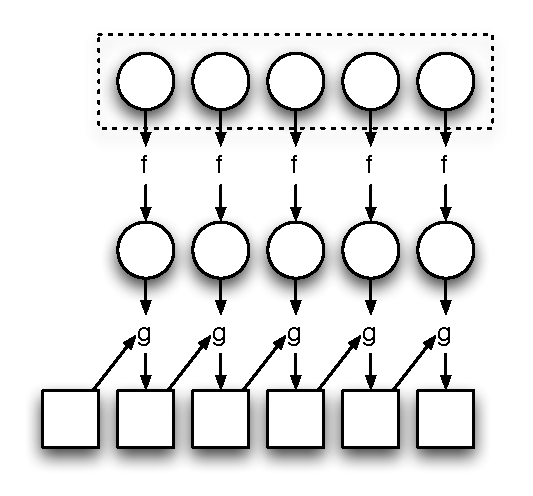
\includegraphics[scale=0.4]{./Figures/functional}
    \caption{Illustration of \emph{map} and \emph{fold}.}
    \label{fig:functional}
  \end{figure}
}

%%%%%%%%%%%%%%%%%%%%%%%%%%%%%%%%%%%%%%%%%%%%%%%%%%%%%%%%%%
\frame {\frametitle{Functional Programming Roots}
%%%%%%%%%%%%%%%%%%%%%%%%%%%%%%%%%%%%%%%%%%%%%%%%%%%%%%%%%%
  \begin{itemize}
  \item \textbf{map phase:}
    \begin{itemize}
    \item Given a list, \emph{map} takes as an argument a function $f$
      (that takes a single argument) and applies it to all element in a list
    \end{itemize}

    \vspace{20pt}

  \item \textbf{fold phase:}
    \begin{itemize}
    \item Given a list, fold takes as arguments a function $g$ (that
      takes two arguments) and an initial value (an accumulator)
    \item $g$ is first applied to the initial value and the first
      item in the list
    \item The result is stored in an intermediate variable, which is
      used as an input together with the next item to a second
      application of $g$
    \item The process is repeated until all items in the list have
      been consumed
    \end{itemize}
 \end{itemize}
}

%%%%%%%%%%%%%%%%%%%%%%%%%%%%%%%%%%%%%%%%%%%%%%%%%%%%%%%%%%
\frame {\frametitle{Functional Programming Roots}
%%%%%%%%%%%%%%%%%%%%%%%%%%%%%%%%%%%%%%%%%%%%%%%%%%%%%%%%%%
  \begin{itemize}
  \item \textbf{We can view map as a transformation over a dataset}
    \begin{itemize}
    \item This transformation is specified by the function $f$
    \item Each functional application happens in
      {\color{red} \textbf{isolation}}
    \item The application of $f$ to each element of a dataset can be
      parallelized in a straightforward manner
    \end{itemize}

    \vspace{20pt}

  \item \textbf{We can view fold as an aggregation operation}
    \begin{itemize}
    \item The aggregation is defined by the function $g$
    \item Data locality: elements in the list must be ``brought
      together''
    \item If we can {\color{red} \textbf{group}} elements of the list, also the fold phase can proceed in parallel 
    \end{itemize}

    \vspace{20pt}

  \item \textbf{Associative and commutative operations}
    \begin{itemize}
    \item Allow performance gains through local aggregation and reordering
    \end{itemize}
  \end{itemize}
 
}

%%%%%%%%%%%%%%%%%%%%%%%%%%%%%%%%%%%%%%%%%%%%%%%%%%%%%%%%%%
\frame {\frametitle{Functional Programming and MapReduce}
%%%%%%%%%%%%%%%%%%%%%%%%%%%%%%%%%%%%%%%%%%%%%%%%%%%%%%%%%%
  \begin{itemize}
  \item \textbf{Equivalence of MapReduce and Functional Programming: }
    \begin{itemize}
    \item The map of MapReduce corresponds to the map operation
    \item The reduce of MapReduce corresponds to the fold operation
    \end{itemize}

    \vspace{20pt}

  \item\textbf{The framework coordinates the map and reduce phases:}
    \begin{itemize}
    \item Grouping intermediate results happens in parallel
    \end{itemize}

    \vspace{20pt}
    
  \item \textbf{In practice:}
    \begin{itemize}
    \item User-specified computation is applied (in parallel) to all input
      records of a dataset
    \item Intermediate results are aggregated by another
      user-specified computation
    \end{itemize}

  \end{itemize}
}

%%%%%%%%%%%%%%%%%%%%%%%%%%%%%%%%%%%%%%%%%%%%%%%%%%%%%%%%%%
\frame {\frametitle{What can we do with MapReduce?}
%%%%%%%%%%%%%%%%%%%%%%%%%%%%%%%%%%%%%%%%%%%%%%%%%%%%%%%%%%
  \begin{itemize}
  \item \textbf{MapReduce ``implements'' a subset of functional
      programming}
    \begin{itemize}
    \item The programming model appears quite limited and strict
    \end{itemize}

\vspace{20pt}

  \item \textbf{There are several important problems that can be
      adapted to MapReduce}
    \begin{itemize}
    \item We will focus on illustrative cases
    \item We will see in detail ``design patterns''
      \begin{itemize}
      \item How to transform a problem and its input
      \item How to save memory and bandwidth in the system
      \end{itemize}
    \end{itemize}

  \end{itemize}

}

%%%%%%%%%%%%%%%%%%%%%%%%%%%%%%%%%%%%%%%%%%%%%%%%%%%%%%%%%%
\frame {\frametitle{Data Structures}
%%%%%%%%%%%%%%%%%%%%%%%%%%%%%%%%%%%%%%%%%%%%%%%%%%%%%%%%%%
  \begin{itemize}
  \item \textbf{Key-value pairs are the basic data structure in
      MapReduce}
    \begin{itemize}
    \item Keys and values can be: integers, float, strings, raw bytes
    \item They can also be \textbf{arbitrary data structures}
    \end{itemize}

    \vspace{20pt}

  \item \textbf{The design of MapReduce algorithms involves}:
    \begin{itemize}
    \item Imposing the key-value structure on arbitrary datasets\footnote{There's more about it: here we only look at the input to the map function.}
      \begin{itemize}
      \item E.g.: for a collection of Web pages, input keys may be URLs
        and values may be the HTML content
      \end{itemize}
    \item In some algorithms, input keys are not used, in others they
      uniquely identify a record
    \item Keys can be combined in complex ways to design various algorithms
    \end{itemize}
  \end{itemize}
}

%%%%%%%%%%%%%%%%%%%%%%%%%%%%%%%%%%%%%%%%%%%%%%%%%%%%%%%%%%
\frame {\frametitle{A Generic MapReduce Algorithm}
%%%%%%%%%%%%%%%%%%%%%%%%%%%%%%%%%%%%%%%%%%%%%%%%%%%%%%%%%%
  \begin{itemize}
  \item \textbf{The programmer defines a mapper and a reducer as
      follows}\footnote{We use the convention $[ \cdots ]$ to denote a list.}\footnote{Pedices indicate different data types.}:
    \begin{itemize}
    \item map: $(k_1,v_1) \to [(k_2,v_2)]$
    \item reduce: $(k_2,[v_2]) \to [(k_3,v_3)]$
    \end{itemize}

    \vspace{20pt}

  \item \textbf{In words}:
    \begin{itemize}
    \item A dataset stored on an underlying \textbf{distributed} filesystem,
      which is split in a number of \textbf{blocks} across machines
    \item The mapper is applied to every input key-value pair to
      generate intermediate key-value pairs
    \item The reducer is applied to all values associated with the
      same intermediate key to generate output key-value pairs
    \end{itemize}
  \end{itemize}
}

%%%%%%%%%%%%%%%%%%%%%%%%%%%%%%%%%%%%%%%%%%%%%%%%%%%%%%%%%%
\frame {\frametitle{Where the magic happens}
%%%%%%%%%%%%%%%%%%%%%%%%%%%%%%%%%%%%%%%%%%%%%%%%%%%%%%%%%%
  \begin{itemize}
  \item \textbf{Implicit between the map and reduce phases is a {\color{red}parallel ``\textbf{group by}''} operation on intermediate keys}
    \begin{itemize}
    \item Intermediate data arrive at each reducer in order, sorted by
      the key
    \item No ordering is guaranteed across reducers
   \end{itemize}

    \vspace{20pt}

  \item \textbf{Output keys from reducers are written back to the
      distributed filesystem}
    \begin{itemize}
    \item The output may consist of $r$ distinct files, where $r$ is
      the number of reducers
    \item Such output may be the input to a subsequent MapReduce phase\footnote{Think of \textbf{iterative algorithms}.}
    \end{itemize}

    \vspace{20pt}

  \item \textbf{Intermediate keys are transient}:
    \begin{itemize}
    \item They are not stored on the distributed filesystem
    \item They are ``spilled'' to the local disk of each machine in
      the cluster
    \end{itemize}
  \end{itemize}
}

%%%%%%%%%%%%%%%%%%%%%%%%%%%%%%%%%%%%%%%%%%%%%%%%%%%%%%%%%%
\frame {\frametitle{``Hello World'' in MapReduce}
%%%%%%%%%%%%%%%%%%%%%%%%%%%%%%%%%%%%%%%%%%%%%%%%%%%%%%%%%%
  \begin{figure}[h]
    \centering
    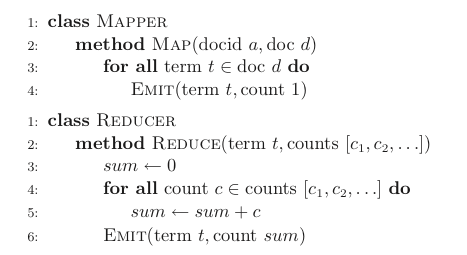
\includegraphics[scale=0.5]{./Figures/word_count}
    \caption{Pseudo-code for the word count algorithm.}
    \label{fig:word_count}
  \end{figure}
}

%%%%%%%%%%%%%%%%%%%%%%%%%%%%%%%%%%%%%%%%%%%%%%%%%%%%%%%%%%
\frame {\frametitle{}
%%%%%%%%%%%%%%%%%%%%%%%%%%%%%%%%%%%%%%%%%%%%%%%%%%%%%%%%%%
  \begin{figure}[h]
    \centering
    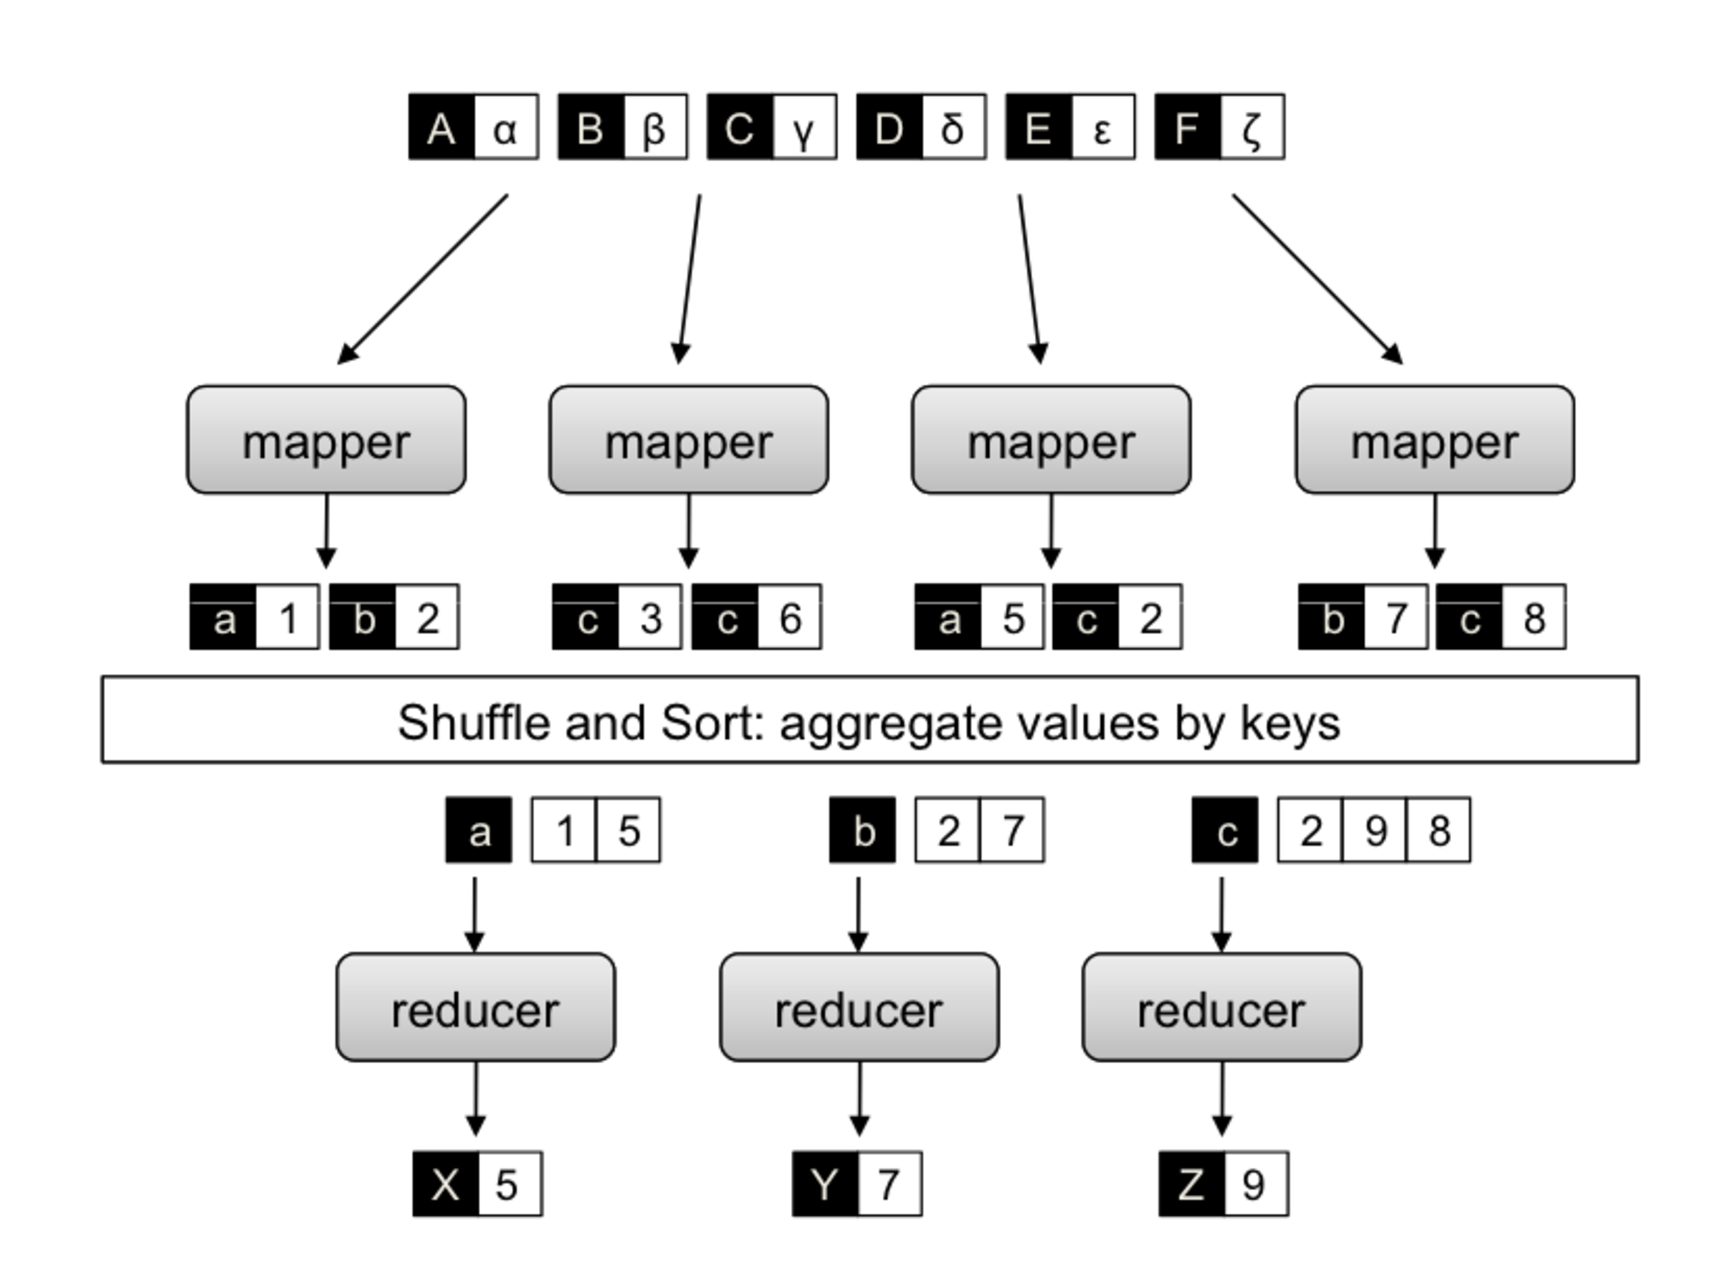
\includegraphics[scale=0.23]{./Figures/simple_MR}
    \label{fig:simple_MR}
  \end{figure}
}

\frame {\frametitle{``Hello World'' in MapReduce}
  \begin{itemize}

  \item \textbf{Input:}
    \begin{itemize}
    \item Key-value pairs: (docid, doc) stored on the distributed filesystem
    \item docid: unique identifier of a document
    \item doc: is the text of the document itself
    \end{itemize}

  \item \textbf{Mapper:}
    \begin{itemize}
    \item Takes an input key-value pair, tokenize the document 
    \item Emits intermediate key-value pairs: the word is the key and
      the integer is the value
    \end{itemize}

  \item \textbf{The framework:}
    \begin{itemize}
    \item Guarantees all values associated with the same key (the
      word) are brought to the same reducer
    \end{itemize}

  \item \textbf{The reducer:}
    \begin{itemize}
    \item Receives all values associated to some keys
    \item Sums the values and writes output key-value pairs: the key
      is the word and the value is the number of occurrences
    \end{itemize}
  \end{itemize}
}

%%%%%%%%%%%%%%%%%%%%%%%%%%%%%%%%%%%%%%%%%%%%%%%%%%%%%%%%%%


%%%%%%%%%%%%%%%%%%%%%%%%%%%%%%%%%%%%%%%%%%%%%%%%%%%%%%%%%%
\section{Basic Design Patterns}

\begin{frame}
 \begin{colorblock}{blue}{lightblue}{ }
  \begin{center}
    \Huge \textbf{\texttt{Basic Design Patterns}}
  \end{center}
  \end{colorblock}
\end{frame}

%%%%%%%%%%%%%%%%%%%%%%%%%%%%%%%%%%%%%%%%%%%%%%%%%%%%%%%%%%
\frame {\frametitle{Algorithm Design}
%%%%%%%%%%%%%%%%%%%%%%%%%%%%%%%%%%%%%%%%%%%%%%%%%%%%%%%%%%
  \begin{itemize}
  \item \textbf{Developing algorithms involve:}
    \begin{itemize}
    \item Preparing the input data
    \item Implement the mapper and the reducer
    \item Optionally, design the combiner and the partitioner
   \end{itemize}

    \vspace{20pt}

  \item \textbf{How to recast existing algorithms in MapReduce?}
    \begin{itemize}
   \item It is not always obvious how to express algorithms
    \item Data structures play an important role
    \item Optimization is hard
    \item[$\to$] The designer needs to ``bend'' the framework
    \end{itemize}

    \vspace{20pt}

  \item \textbf{Learn by examples}
    \begin{itemize}
    \item ``Design patterns''
    \item ``Shuffle'' is perhaps the most tricky aspect
    \end{itemize}
  \end{itemize}
}

%%%%%%%%%%%%%%%%%%%%%%%%%%%%%%%%%%%%%%%%%%%%%%%%%%%%%%%%%%
\frame {\frametitle{Algorithm Design}
%%%%%%%%%%%%%%%%%%%%%%%%%%%%%%%%%%%%%%%%%%%%%%%%%%%%%%%%%%
  \begin{itemize}
  \item \textbf{Aspects that are {\color{red}not} under the control of the
    designer}
    \begin{itemize}
    \item \textit{Where} a mapper or reducer will run
    \item \textit{When} a mapper or reducer begins or finishes
    \item \textit{Which} input key-value pairs are processed by a
      specific mapper
    \item \textit{Which} intermediate key-value pairs are processed by a
      specific reducer
    \end{itemize}

    \vspace{20pt}

  \item \textbf{Aspects that can be controlled}
    \begin{itemize}
    \item Construct {\color{red}data structures as keys and values}
    \item Execute user-specified initialization and termination code
      for mappers and reducers
    \item Preserve state across multiple input and intermediate keys
      in mappers and reducers
    \item {\color{red}Control the sort order} of intermediate keys, and therefore
      the order in which a reducer will encounter particular keys
    \item {\color{red}Control the partitioning of the key space}, and therefore the
      set of keys that will be encountered by a particular reducer
    \end{itemize}
  \end{itemize}
}

%%%%%%%%%%%%%%%%%%%%%%%%%%%%%%%%%%%%%%%%%%%%%%%%%%%%%%%%%%
\frame {\frametitle{Algorithm Design}
%%%%%%%%%%%%%%%%%%%%%%%%%%%%%%%%%%%%%%%%%%%%%%%%%%%%%%%%%%
  \begin{itemize}
  \item \textbf{MapReduce algorithms can be complex}
    \begin{itemize}
    \item Many algorithms cannot be easily expressed as a single
      MapReduce job
    \item Decompose complex algorithms into a sequence of jobs
      \begin{itemize}
      \item Requires orchestrating data so that the output of one job
        becomes the input to the next
      \end{itemize}
    \item Iterative algorithms require an {\color{red}external driver}
      to check for convergence
    \end{itemize}

    \vspace{20pt}

  \item \textbf{Basic design patterns\footnote{You will see them in action during the laboratory sessions.}}
    \begin{itemize}
    \item Local Aggregation
    \item Pairs and Stripes
    \item Order inversion
    \end{itemize}
 \end{itemize}
}

%%%%%%%%%%%%%%%%%%%%%%%%%%%%%%%%%%%%%%%%%%%%%%%%%%%%%%%%%%
%%%%%%%%%%%%%%%%%%%%%%%%%%%%%%%%%%%%%%%%%%%%%%%%%%%%%%%%%%
\subsection{Local Aggregation}
%%%%%%%%%%%%%%%%%%%%%%%%%%%%%%%%%%%%%%%%%%%%%%%%%%%%%%%%%%
%%%%%%%%%%%%%%%%%%%%%%%%%%%%%%%%%%%%%%%%%%%%%%%%%%%%%%%%%%


%%%%%%%%%%%%%%%%%%%%%%%%%%%%%%%%%%%%%%%%%%%%%%%%%%%%%%%%%%
\frame {\frametitle{Local Aggregation}
%%%%%%%%%%%%%%%%%%%%%%%%%%%%%%%%%%%%%%%%%%%%%%%%%%%%%%%%%%
  \begin{itemize}
  \item \textbf{In the context of data-intensive distributed processing, the
      most important aspect of synchronization is the {\color{red}exchange of
        intermediate results}}
    \begin{itemize}
    \item This involves copying intermediate results from the
      processes that produced them to those that consume them
    \item In general, this involves \textbf{data transfers over the network}
    \item In Hadoop, also disk I/O is involved, as intermediate
      results are written to disk
    \end{itemize}

    \vspace{20pt}

    \item \textbf{Network and disk latencies are expensive}
      \begin{itemize}
      \item Reducing the amount of intermediate data translates into
        algorithmic efficiency
      \end{itemize}

      \vspace{20pt}

    \item \textbf{Combiners and preserving state across inputs}
      \begin{itemize}
      \item Reduce the number and size of key-value pairs to be shuffled
      \end{itemize}

  \end{itemize}
}


%%%%%%%%%%%%%%%%%%%%%%%%%%%%%%%%%%%%%%%%%%%%%%%%%%%%%%%%%%
\frame {\frametitle{In-Mapper Combiners}
%%%%%%%%%%%%%%%%%%%%%%%%%%%%%%%%%%%%%%%%%%%%%%%%%%%%%%%%%%
  \begin{itemize}
  \item \textbf{In-Mapper Combiners, a possible improvement over vanilla Combiners}
    \begin{itemize}
    \item Hadoop does not\footnote{Actually, combiners are not called if the number of map output records is less than a small threshold, {\it i.e.}, 4} guarantee combiners to be executed
    \end{itemize}

    \vspace{20pt}

  \item \textbf{Use an associative array to cumulate intermediate
      results}
    \begin{itemize}
    \item The array is used to tally up term counts within a single ``document''
    \item The \texttt{Emit} method is called only after all \texttt{InputRecords} have been processed
    \end{itemize}

    \vspace{20pt}

  \item \textbf{Example (see next slide)}
    \begin{itemize}
    \item The code emits a key-value pair for each {\color{red}unique}
      term in the document
    \end{itemize}
  \end{itemize}
}

%%%%%%%%%%%%%%%%%%%%%%%%%%%%%%%%%%%%%%%%%%%%%%%%%%%%%%%%%%
\frame {\frametitle{In-Memory Combiners}
%%%%%%%%%%%%%%%%%%%%%%%%%%%%%%%%%%%%%%%%%%%%%%%%%%%%%%%%%%
\begin{algorithm}[H]
\algrenewcommand\algorithmicfunction{\textbf{class}}
\algrenewcommand\algorithmicprocedure{\textbf{method}}

  \begin{algorithmic}[1]
    \Function{Mapper}{}
    \Procedure{Map}{offset $a$, line $l$}
    \State $H \gets$  new AssociativeArray
    \ForAll{term $t \in$ line $l$}
      \State $H\{t\} \gets H\{t\} + 1$
    \EndFor
    \ForAll{term $t \in$ $H$}
      \State $\textsc{Emit}(\textrm{term }t, \textrm{count }H\{t\})$
    \EndFor
    \EndProcedure
    \EndFunction
  \end{algorithmic}
\end{algorithm}

}

\frame {\frametitle{In-Memory Combiners}
  \begin{itemize}
  \item \textbf{Taking the idea one step further}
    \begin{itemize}
    \item Exploit implementation details in Hadoop
    \item A Java mapper object is created for each map task
    \item JVM reuse must be enabled
    \end{itemize}

    \vspace{40pt}

  \item \textbf{Preserve state within and across calls to the \texttt{Map}
    method}
    \begin{itemize}
    \item \texttt{Initialize} method, used to create an across-map, persistent
      data structure
    \item \texttt{Close} method, used to emit intermediate key-value
      pairs only when all map task scheduled on one machine are done
    \end{itemize}
  \end{itemize}
}

%%%%%%%%%%%%%%%%%%%%%%%%%%%%%%%%%%%%%%%%%%%%%%%%%%%%%%%%%%
\frame {\frametitle{In-Memory Combiners}
%%%%%%%%%%%%%%%%%%%%%%%%%%%%%%%%%%%%%%%%%%%%%%%%%%%%%%%%%%
\begin{algorithm}[H]
\algrenewcommand\algorithmicfunction{\textbf{class}}
\algrenewcommand\algorithmicprocedure{\textbf{method}}

  \begin{algorithmic}[1]
    \Function{Mapper}{}
      \Procedure{Initialize}{}
        \State $H \gets$  new AssociativeArray
      \EndProcedure
      \Procedure{Map}{offset $a$, line $l$}
        \ForAll{term $t \in$ line $l$}
          \State $H\{t\} \gets H\{t\} + 1$
        \EndFor
      \EndProcedure
      \Procedure{Close}{}
        \ForAll{term $t \in$ $H$}
          \State $\textsc{Emit}(\textrm{term }t, \textrm{count }H\{t\})$
        \EndFor
      \EndProcedure
    \EndFunction
  \end{algorithmic}
\end{algorithm}

}

%%%%%%%%%%%%%%%%%%%%%%%%%%%%%%%%%%%%%%%%%%%%%%%%%%%%%%%%%%
\frame {\frametitle{In-Memory Combiners}
%%%%%%%%%%%%%%%%%%%%%%%%%%%%%%%%%%%%%%%%%%%%%%%%%%%%%%%%%%
  \begin{itemize}
  \item \textbf{Summing up: a first ``design pattern'', \textit{in-memory
        combining}}
    \begin{itemize}
    \item Provides control over when local aggregation occurs
    \item Designer can determine how exactly aggregation is done
    \end{itemize}

    \vspace{40pt}

  \item \textbf{Efficiency vs. Combiners}
    \begin{itemize}
    \item There is no additional overhead due to the materialization
      of key-value pairs
      \begin{itemize}
      \item Un-necessary object creation and destruction (garbage
        collection)
      \item Serialization, deserialization when memory bounded
      \end{itemize}
    \item With combiners. mappers still need to emit all key-value pairs, combiners
      ``only'' reduce network traffic
    \end{itemize}
  \end{itemize}
}

%%%%%%%%%%%%%%%%%%%%%%%%%%%%%%%%%%%%%%%%%%%%%%%%%%%%%%%%%%
\frame {\frametitle{In-Memory Combiners}
%%%%%%%%%%%%%%%%%%%%%%%%%%%%%%%%%%%%%%%%%%%%%%%%%%%%%%%%%%
  \begin{itemize}
  \item \textbf{Precautions}
    \begin{itemize}
    \item In-memory combining breaks the functional programming
      paradigm due to {\bf state preservation}
    \item Preserving state across multiple instances implies that
      algorithm behavior might depend on execution order
      \begin{itemize}
      \item Works well with commutative / associative operations
      \item Otherwise, order-dependent bugs are difficult to find
      \end{itemize}
    \end{itemize}

    \vspace{20pt}

  \item \textbf{Memory capacity is limited}
    \begin{itemize}
    \item In-memory combining strictly depends on having sufficient memory to store intermediate results
    \item A possible {\color{red}solution}: ``block'' and ``flush''
    \end{itemize}
  \end{itemize}
}

%%%%%%%%%%%%%%%%%%%%%%%%%%%%%%%%%%%%%%%%%%%%%%%%%%%%%%%%%%
\frame {\frametitle{Further Remarks}
%%%%%%%%%%%%%%%%%%%%%%%%%%%%%%%%%%%%%%%%%%%%%%%%%%%%%%%%%%
  \begin{itemize}
  \item \textbf{The extent to which efficiency can be increased with local
      aggregation depends on the size of the intermediate key space}
    \begin{itemize}
    \item Opportunities for aggregation arise when multiple values
      are associated to the same keys
    \end{itemize}

    \vspace{40pt}

  \item \textbf{Local aggregation also effective to deal with reduce
      stragglers}
    \begin{itemize}
    \item Reduce the number of values associated with frequently occurring keys
    \end{itemize}
  \end{itemize}
}


%%%%%%%%%%%%%%%%%%%%%%%%%%%%%%%%%%%%%%%%%%%%%%%%%%%%%%%%%%
\frame {\frametitle{Computing the average, with in-mapper combiners}
%%%%%%%%%%%%%%%%%%%%%%%%%%%%%%%%%%%%%%%%%%%%%%%%%%%%%%%%%%
  \begin{itemize}
    \item Partial sums and counts are held in memory (across inputs)
    \item Intermediate values are emitted only after the entire input
      split is processed
    \item The output value is a pair
  \end{itemize}

\begin{algorithm}[H]
\algrenewcommand\algorithmicfunction{\textbf{class}}
\algrenewcommand\algorithmicprocedure{\textbf{method}}

  \begin{algorithmic}[1]
    \Function{Mapper}{}
      \Procedure{Initialize}{}
        \State $S \gets$  new AssociativeArray
        \State $C \gets$  new AssociativeArray
      \EndProcedure
      \Procedure{Map}{term $t$, integer $r$}
        \State $S\{t\} \gets S\{t\} + r$
        \State $C\{t\} \gets C\{t\} + 1$
      \EndProcedure
      \Procedure{Close}{}
        \ForAll{term $t \in$ $S$}
          \State $\textsc{Emit}(\textrm{term }t, \textrm{pair }(S\{t\},C\{t\}))$
        \EndFor
      \EndProcedure
    \EndFunction
  \end{algorithmic}
\end{algorithm}

} 

%%%%%%%%%%%%%%%%%%%%%%%%%%%%%%%%%%%%%%%%%%%%%%%%%%%%%%%%%%
%%%%%%%%%%%%%%%%%%%%%%%%%%%%%%%%%%%%%%%%%%%%%%%%%%%%%%%%%%
\subsection{Pairs and Stripes}
%%%%%%%%%%%%%%%%%%%%%%%%%%%%%%%%%%%%%%%%%%%%%%%%%%%%%%%%%%
%%%%%%%%%%%%%%%%%%%%%%%%%%%%%%%%%%%%%%%%%%%%%%%%%%%%%%%%%%

%%%%%%%%%%%%%%%%%%%%%%%%%%%%%%%%%%%%%%%%%%%%%%%%%%%%%%%%%%
\frame {\frametitle{Pairs and Stripes}
%%%%%%%%%%%%%%%%%%%%%%%%%%%%%%%%%%%%%%%%%%%%%%%%%%%%%%%%%%
  \begin{itemize}
  \item \textbf{A common approach in MapReduce: build {\color{red}complex} keys}
    \begin{itemize}
    \item Use the framework to group data together
    \end{itemize}

    \vspace{20pt}

  \item \textbf{Two basic techniques:}
   \begin{itemize}
    \item \textit{Pairs}: similar to the example on the average
    \item \textit{Stripes}: uses in-mapper memory data structures
    \end{itemize}

    \vspace{20pt}

  \item \textbf{Next, we focus on a particular problem that benefits
      from these two methods}
 \end{itemize}
}

%%%%%%%%%%%%%%%%%%%%%%%%%%%%%%%%%%%%%%%%%%%%%%%%%%%%%%%%%%
\frame {\frametitle{Problem statement}
%%%%%%%%%%%%%%%%%%%%%%%%%%%%%%%%%%%%%%%%%%%%%%%%%%%%%%%%%%
  \begin{itemize}
  \item \textbf{The problem: building word co-occurrence matrices for large corpora}
    \begin{itemize}
    \item The co-occurrence matrix of a corpus is a square $n \times n$ matrix, $M$
    \item $n$ is the number of unique words (\textit{i.e.}, the vocabulary size)
    \item A cell $m_{ij}$ contains the number of times the word $w_i$ co-occurs with word $w_j$ \textit{within a specific context}
    \item Context: a sentence, a paragraph a document or a window of $m$ words
    \item NOTE: the matrix may be symmetric in some cases
    \end{itemize}

    \vspace{20pt}

  \item \textbf{Motivation}
    \begin{itemize}
    \item This problem is a basic building block for more complex operations
    \item {\color{red}Estimating the distribution of discrete joint events from a large number of observations}
    \item Similar problem in other domains:
      \begin{itemize}
      \item Customers who buy \textit{this} tend to also buy
        \textit{that}
      \end{itemize}
    \end{itemize}
  \end{itemize}
}

%%%%%%%%%%%%%%%%%%%%%%%%%%%%%%%%%%%%%%%%%%%%%%%%%%%%%%%%%%
\frame {\frametitle{Observations}
%%%%%%%%%%%%%%%%%%%%%%%%%%%%%%%%%%%%%%%%%%%%%%%%%%%%%%%%%%
  \begin{itemize}
  \item \textbf{Space requirements}
    \begin{itemize}
    \item Clearly, the space requirement is $O(n^2)$, where $n$ is the size of the vocabulary
    \item For real-world (English) corpora $n$ can be hundreds of thousands of words, or even billions of worlds in some specific cases
    \end{itemize}

    \vspace{20pt}

  \item \textbf{So what's the problem?}
    \begin{itemize}
    \item If the matrix can fit in the memory of a single machine, then just use whatever naive implementation
    \item Instead, if the matrix is bigger than the available memory, then {\color{red}paging} would kick in, and any naive
      implementation would break
    \end{itemize}

    \vspace{20pt}

  \item \textbf{Compression}
    \begin{itemize}
    \item Such techniques can help in solving the problem on a single machine
    \item However, there are scalability problems
    \end{itemize}
  \end{itemize}
}

%%%%%%%%%%%%%%%%%%%%%%%%%%%%%%%%%%%%%%%%%%%%%%%%%%%%%%%%%%
\frame {\frametitle{Word co-occurrence: the Pairs approach}
%%%%%%%%%%%%%%%%%%%%%%%%%%%%%%%%%%%%%%%%%%%%%%%%%%%%%%%%%%
  \begin{center}
    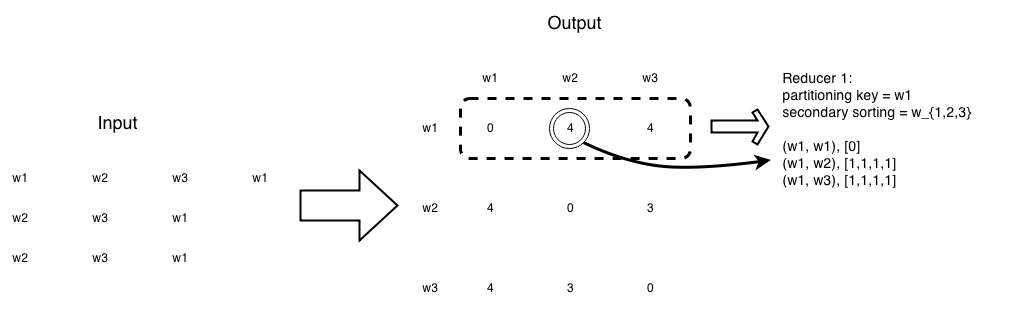
\includegraphics[scale=0.36]{./Figures/pairs}
  \end{center}
}

%%%%%%%%%%%%%%%%%%%%%%%%%%%%%%%%%%%%%%%%%%%%%%%%%%%%%%%%%%
\frame {\frametitle{Word co-occurrence: the Pairs approach}
%%%%%%%%%%%%%%%%%%%%%%%%%%%%%%%%%%%%%%%%%%%%%%%%%%%%%%%%%%
  \begin{itemize}
  \item \textbf{Input to the problem}
    \begin{itemize}
    \item Key-value pairs in the form of a \texttt{offset} and a \texttt{line}
    \end{itemize}

    \vspace{20pt}

  \item \textbf{The mapper:}
    \begin{itemize}
    \item Processes each input document
      \item Emits key-value pairs with:
        \begin{itemize}
        \item Each co-occurring word {\color{red}pair} as the key
        \item The integer one (the count) as the value
        \end{itemize}
      \item This is done with two nested loops:
        \begin{itemize}
        \item The outer loop iterates over all words
        \item The inner loop iterates over all neighbors
        \end{itemize}
    \end{itemize}

    \vspace{20pt}

  \item \textbf{The reducer:}
    \begin{itemize}
    \item Receives {\color{red}pairs} related to co-occurring words
      \begin{itemize}
      \item This {\color{red}requires \textbf{modifying the partitioner}}
      \end{itemize}
    \item Computes an absolute count of the joint event
    \item Emits the pair and the count as the final key-value output
      \begin{itemize}
      \item Basically reducers emit the cells of the output matrix
      \end{itemize}
    \end{itemize}
  \end{itemize}
}

%%%%%%%%%%%%%%%%%%%%%%%%%%%%%%%%%%%%%%%%%%%%%%%%%%%%%%%%%%
\frame {\frametitle{Word co-occurrence: the Pairs approach}
%%%%%%%%%%%%%%%%%%%%%%%%%%%%%%%%%%%%%%%%%%%%%%%%%%%%%%%%%%
\begin{algorithm}[H]
\algrenewcommand\algorithmicfunction{\textbf{class}}
\algrenewcommand\algorithmicprocedure{\textbf{method}}

  \begin{algorithmic}[1]
    \Function{Mapper}{}
      \Procedure{Map}{offset $a$, line $l$}
        \ForAll{term $w \in$ line $l$}
          \ForAll{term $u \in \textsc{Neighbors}(w)$}
            \State $\textsc{Emit } (\textrm{pair }(w,u), \textrm{count }1)$
          \EndFor
        \EndFor
      \EndProcedure
    \EndFunction

    \Function{Reducer}{}
      \Procedure{Reduce}{pair $p$, counts $[c_1,c_2, \cdots ]$}
        \State $s \gets 0$
        \ForAll{count $c \in \textrm{counts }[c_1,c_2, \cdots ]$}
          \State $s \gets s + c$
        \EndFor
        \State $\textsc{Emit } (\textrm{pair }p, \textrm{count }s)$
      \EndProcedure
    \EndFunction

  \end{algorithmic}
\end{algorithm}
}

%%%%%%%%%%%%%%%%%%%%%%%%%%%%%%%%%%%%%%%%%%%%%%%%%%%%%%%%%%
\frame {\frametitle{Word co-occurrence: the Stripes approach}
%%%%%%%%%%%%%%%%%%%%%%%%%%%%%%%%%%%%%%%%%%%%%%%%%%%%%%%%%%
  \begin{center}
    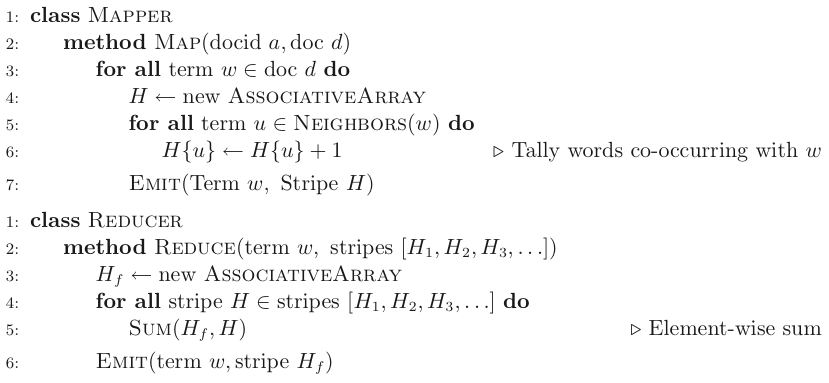
\includegraphics[scale=0.36]{./Figures/stripes}
  \end{center}
}

%%%%%%%%%%%%%%%%%%%%%%%%%%%%%%%%%%%%%%%%%%%%%%%%%%%%%%%%%%
\frame {\frametitle{Word co-occurrence: the Stripes approach}
%%%%%%%%%%%%%%%%%%%%%%%%%%%%%%%%%%%%%%%%%%%%%%%%%%%%%%%%%%
  \begin{itemize}
  \item \textbf{Input to the problem}
    \begin{itemize}
    \item Key-value pairs in the form of a \texttt{offset} and a \texttt{line}
    \end{itemize}

    \vspace{20pt}

  \item \textbf{The mapper:}
    \begin{itemize}
    \item Same two nested loops structure as before
    \item Co-occurrence information is first stored in an associative
      array
    \item Emit key-value pairs with {\color{red}words} as keys and the
      corresponding arrays as values
    \end{itemize}

    \vspace{20pt}

  \item \textbf{The reducer:}
    \begin{itemize}
    \item Receives all associative arrays related to the same word
    \item Performs an element-wise sum of all associative arrays with
      the same key
    \item Emits key-value output in the form of word, associative
      array
      \begin{itemize}
      \item Basically, reducers emit \textbf{rows} of the co-occurrence matrix
      \end{itemize}
    \end{itemize}
 \end{itemize}

}

%%%%%%%%%%%%%%%%%%%%%%%%%%%%%%%%%%%%%%%%%%%%%%%%%%%%%%%%%%
\frame {\frametitle{Word co-occurrence: the Stripes approach}
%%%%%%%%%%%%%%%%%%%%%%%%%%%%%%%%%%%%%%%%%%%%%%%%%%%%%%%%%%
\begin{algorithm}[H]
\algrenewcommand\algorithmicfunction{\textbf{class}}
\algrenewcommand\algorithmicprocedure{\textbf{method}}

  \begin{algorithmic}[1]
    \Function{Mapper}{}
      \Procedure{Map}{offset $a$, line $l$}
        \ForAll{term $w \in$ line $l$}
        \State $H \gets$ new AssociativeArray
          \ForAll{term $u \in \textsc{Neighbors}(w)$}
            \State $H\{u\} \gets H\{u\}+1$
          \EndFor
          \State $\textsc{Emit } (\textrm{term }w, \textrm{Stripe }H)$
        \EndFor
      \EndProcedure
    \EndFunction

    \Function{Reducer}{}
      \Procedure{Reduce}{term $w$, Stripes $[H_1,H_2,H_3 \cdots ]$}
        \State $H_f \gets$ new AssociativeArray
        \ForAll{Stripe $H \in \textrm{Stripes }[H_1,H_2,H_3 \cdots ]$}
          \State $\textsc{Sum}(H_f,H)$
        \EndFor
        \State $\textsc{Emit } (\textrm{term }w, \textrm{Stripe }H_f)$
      \EndProcedure
    \EndFunction

  \end{algorithmic}
\end{algorithm}

}

%%%%%%%%%%%%%%%%%%%%%%%%%%%%%%%%%%%%%%%%%%%%%%%%%%%%%%%%%%
\frame {\frametitle{Pairs and Stripes, a comparison}
%%%%%%%%%%%%%%%%%%%%%%%%%%%%%%%%%%%%%%%%%%%%%%%%%%%%%%%%%%
  \begin{itemize}
  \item \textbf{The pairs approach}
    \begin{itemize}
    \item Generates a large number of key-value pairs
    \begin{itemize}
      \item In particular, intermediate ones, that fly over the network
    \end{itemize}
    \item The benefit from combiners is limited, as it is less likely
      for a mapper to process multiple occurrences of a word
    \item Does not suffer from memory paging problems
    \end{itemize}

    \vspace{20pt}
    
  \item \textbf{The stripes approach}
    \begin{itemize}
    \item More compact
    \item Generates fewer and shorted intermediate keys
      \begin{itemize}
      \item The framework has less sorting to do
      \end{itemize}
    \item The values are more complex and have serialization / deserialization overhead
    \item Greatly benefits from combiners, as the key space is the vocabulary
    \item Suffers from memory paging problems, if not properly engineered
    \end{itemize}
  \end{itemize}
}

%%%%%%%%%%%%%%%%%%%%%%%%%%%%%%%%%%%%%%%%%%%%%%%%%%%%%%%%%%
%%%%%%%%%%%%%%%%%%%%%%%%%%%%%%%%%%%%%%%%%%%%%%%%%%%%%%%%%%
\subsection{Order Inversion}
%%%%%%%%%%%%%%%%%%%%%%%%%%%%%%%%%%%%%%%%%%%%%%%%%%%%%%%%%%
%%%%%%%%%%%%%%%%%%%%%%%%%%%%%%%%%%%%%%%%%%%%%%%%%%%%%%%%%%

%%%%%%%%%%%%%%%%%%%%%%%%%%%%%%%%%%%%%%%%%%%%%%%%%%%%%%%%%%
\frame {\frametitle{Computing relative frequencies}
%%%%%%%%%%%%%%%%%%%%%%%%%%%%%%%%%%%%%%%%%%%%%%%%%%%%%%%%%%
  \begin{itemize}
  \item \textbf{``Relative'' Co-occurrence matrix construction}
    \begin{itemize}
    \item Similar problem as before, same matrix
    \item Instead of absolute counts, we take into consideration the
      fact that some words appear more frequently than others
      \begin{itemize}
      \item Word $w_i$ may co-occur frequently with word $w_j$ simply
        because one of the two is very common
      \end{itemize}
    \item We need to convert absolute counts to relative frequencies
      $f(w_j | w_i)$
      \begin{itemize}
      \item What proportion of the time does $w_j$ appear in the
        context of $w_i$?
      \end{itemize}
    \end{itemize}

    \vspace{20pt}

  \item \textbf{Formally, we compute:}
    $$ f(w_j | w_i) = \frac{N(w_i,w_j)}{\sum_{w'} N(w_i, w')}$$
    \begin{itemize}
    \item $N(\cdot,\cdot)$ is the number of times a co-occurring word
      pair is observed
    \item The denominator is called the marginal
    \end{itemize}


  \end{itemize}
}

%%%%%%%%%%%%%%%%%%%%%%%%%%%%%%%%%%%%%%%%%%%%%%%%%%%%%%%%%%
\frame {\frametitle{Computing relative frequencies}
%%%%%%%%%%%%%%%%%%%%%%%%%%%%%%%%%%%%%%%%%%%%%%%%%%%%%%%%%%
  \begin{itemize}
  \item \textbf{The stripes approach}
    \begin{itemize}
    \item In the reducer, the counts of all words that co-occur with
      the conditioning variable ($w_i$) are available in the
      associative array
    \item Hence, the sum of all those counts gives the marginal
    \item Then we divide the joint counts by the marginal and
      we're done
    \end{itemize}

    \vspace{40pt}

  \item \textbf{The pairs approach}
    \begin{itemize}
    \item The reducer receives the pair $(w_i,w_j)$ and the count
    \item From this information alone \textbf{it is not possible} to compute
      $f(w_j | w_i)$
    \item Fortunately, as for the mapper, also the reducer can
      {\color{red}preserve state} across multiple keys
      \begin{itemize}
      \item We can buffer in memory all the words that co-occur with
        $w_i$ and their counts
      \item This is basically building the associative array in the
        stripes method
      \end{itemize}
    \end{itemize}
  \end{itemize}
}

%%%%%%%%%%%%%%%%%%%%%%%%%%%%%%%%%%%%%%%%%%%%%%%%%%%%%%%%%%
\frame {\frametitle{Computing relative frequencies: a basic approach}
%%%%%%%%%%%%%%%%%%%%%%%%%%%%%%%%%%%%%%%%%%%%%%%%%%%%%%%%%%
  \begin{itemize}
  \item \textbf{We must define the sort order of the pair}
    \begin{itemize}
    \item In this way, the keys are first sorted by the left word, and
      then by the right word (in the pair)
    \item Hence, we can detect if all pairs associated with the word
      we are conditioning on ($w_i$) have been seen
    \item At this point, we can use the in-memory buffer, compute the
      relative frequencies and emit
    \end{itemize}

    \vspace{20pt}

  \item \textbf{We must define an appropriate partitioner}
    \begin{itemize}
    \item The default partitioner is based on the hash value of the
      intermediate key, modulo the number of reducers
    \item For a complex key, the {\bf raw byte representation} is used to
      compute the hash value
      \begin{itemize}
      \item Hence, there is no guarantee that the pair (dog, aardvark)
        and (dog,zebra) are sent to the same reducer
      \end{itemize}
    \item What we want is that all pairs with the same left word are
      sent to the same reducer
   \end{itemize}

    \vspace{20pt}

  \item \textbf{Limitations of this approach}
    \begin{itemize}
    \item Essentially, we reproduce the stripes method in the reducer
      and we need to use a custom partitioner
    \item This algorithm would work, but present the same
      memory-bottleneck problem as the stripes method
    \end{itemize}
  \end{itemize}
}

%%%%%%%%%%%%%%%%%%%%%%%%%%%%%%%%%%%%%%%%%%%%%%%%%%%%%%%%%%
\frame {\frametitle{Computing relative frequencies: order inversion}
%%%%%%%%%%%%%%%%%%%%%%%%%%%%%%%%%%%%%%%%%%%%%%%%%%%%%%%%%%
  \begin{itemize}
  \item \textbf{The key is to properly sequence data presented to
      reducers}
    \begin{itemize}
    \item If it were possible to compute the marginal in the reducer
      before processing the joint counts, the reducer could simply
      divide the joint counts received from mappers by the marginal
    \item The notion of ``before'' and ``after'' can be captured in
      the {\color{red}ordering of key-value pairs}
    \item The programmer can define the sort order of keys so that
      data needed earlier is presented to the reducer before data that
      is needed later
    \end{itemize}
\end{itemize}
}

%%%%%%%%%%%%%%%%%%%%%%%%%%%%%%%%%%%%%%%%%%%%%%%%%%%%%%%%%%
\frame {\frametitle{Computing relative frequencies: order inversion}
%%%%%%%%%%%%%%%%%%%%%%%%%%%%%%%%%%%%%%%%%%%%%%%%%%%%%%%%%%
  \begin{itemize}
  \item \textbf{Recall that mappers emit pairs of co-occurring words
      as keys}

    \vspace{20pt}

  \item \textbf{The mapper:}
    \begin{itemize}
    \item additionally emits a ``special'' key of the form $(w_i,*)$
    \item The value associated to the special key is one, that
      represents the contribution of the word pair to the marginal
    \item Using combiners, these partial marginal counts will be
      aggregated before being sent to the reducers
    \end{itemize}

    \vspace{20pt}

  \item \textbf{The reducer:}
    \begin{itemize}
    \item We must make sure that the special key-value pairs are
      processed {\color{red}before} any other key-value pairs where
      the left word is $w_i$
    \item We also need to modify the partitioner as before,
      \textit{i.e.}, it would take into account only the first word
    \end{itemize}
  \end{itemize}
}


%%%%%%%%%%%%%%%%%%%%%%%%%%%%%%%%%%%%%%%%%%%%%%%%%%%%%%%%%%
\frame {\frametitle{Computing relative frequencies: order inversion}
%%%%%%%%%%%%%%%%%%%%%%%%%%%%%%%%%%%%%%%%%%%%%%%%%%%%%%%%%%
  \begin{itemize}
  \item \textbf{Memory requirements:}
    \begin{itemize}
    \item Minimal, because only the marginal (an integer) needs to be
      stored
    \item No buffering of individual co-occurring word
    \item No scalability bottleneck
    \end{itemize}

    \vspace{20pt}

  \item \textbf{Key ingredients for order inversion}
    \begin{itemize}
    \item Emit a special key-value pair to capture the marginal
    \item Control the sort order of the intermediate key, so that the
      special key-value pair is processed first
    \item Define a custom partitioner for routing intermediate
      key-value pairs
    \item Preserve state across multiple keys in the reducer
    \end{itemize}
  \end{itemize}
}

%%%%%%%%%%%%%%%%%%%%%%%%%%%%%%%%%%%%%%%%%%%%%%%%%%%%%%%%%%


%%%%%%%%%%%%%%%%%%%%%%%%%%%%%%%%%%%%%%%%%%%%%%%%%%%%%%%%%%
\section{Graph Algorithms}

\begin{frame}
 \begin{colorblock}{blue}{lightblue}{ }
  \begin{center}
    \Huge \textbf{\texttt{Graph Algorithms [Optional]}}
  \end{center}
  \end{colorblock}
\end{frame}

%%%%%%%%%%%%%%%%%%%%%%%%%%%%%%%%%%%%%%%%%%%%%%%%%%%%%%%%%%
%%%%%%%%%%%%%%%%%%%%%%%%%%%%%%%%%%%%%%%%%%%%%%%%%%%%%%%%%%
\subsection{Preliminaries}
%%%%%%%%%%%%%%%%%%%%%%%%%%%%%%%%%%%%%%%%%%%%%%%%%%%%%%%%%%
%%%%%%%%%%%%%%%%%%%%%%%%%%%%%%%%%%%%%%%%%%%%%%%%%%%%%%%%%%


%%%%%%%%%%%%%%%%%%%%%%%%%%%%%%%%%%%%%%%%%%%%%%%%%%%%%%%%%%
\frame {\frametitle{Motivations}
%%%%%%%%%%%%%%%%%%%%%%%%%%%%%%%%%%%%%%%%%%%%%%%%%%%%%%%%%%
  \begin{itemize}
  \item \textbf{Examples of graph problems}
    \begin{itemize}
    \item Clustering
    \item Matching problems
    \item Element analysis: node and edge centralities
    \end{itemize}

    \vspace{20pt}
    
  \item \textbf{The problem: big graphs}

    \vspace{20pt}
    
  \item \textbf{Why MapReduce?}
    \begin{itemize}
    \item Algorithms for the above problems on a single machine are
      not scalable
    \item Recently, Google designed a new system, Pregel, for
      large-scale ({\color{red}incremental}) graph processing
    \item Even more recently, \cite{Lattanzi2011} indicate a
      fundamentally new design pattern to analyze graphs in MapReduce
    \item New trend: graph databases, graph processing systems\footnote{If you're interested, we'll discuss this off-line.}
    \end{itemize}
  \end{itemize}
}

%%%%%%%%%%%%%%%%%%%%%%%%%%%%%%%%%%%%%%%%%%%%%%%%%%%%%%%%%%
\frame {\frametitle{Graph Representations}
%%%%%%%%%%%%%%%%%%%%%%%%%%%%%%%%%%%%%%%%%%%%%%%%%%%%%%%%%%
  \begin{itemize}
  \item \textbf{Basic data structures}
    \begin{itemize}
    \item Adjacency matrix
    \item Adjacency list
    \end{itemize}

    \vspace{20pt}

  \item \textbf{Are graphs sparse or dense?}
    \begin{itemize}
    \item Determines which data-structure to use
      \begin{itemize}
      \item Adjacency matrix: operations on incoming links are easy
        (column scan)
      \item Adjacency list: operations on outgoing links are easy
      \item The shuffle and sort phase can help, by grouping edges by
        their destination reducer
      \end{itemize}
    \item \cite{Leskovec2005} dispelled the notion of sparseness of real-world graphs
    \end{itemize}
  \end{itemize}
}

%%%%%%%%%%%%%%%%%%%%%%%%%%%%%%%%%%%%%%%%%%%%%%%%%%%%%%%%%%
%%%%%%%%%%%%%%%%%%%%%%%%%%%%%%%%%%%%%%%%%%%%%%%%%%%%%%%%%%
\subsection{Breadth-First Search}
%%%%%%%%%%%%%%%%%%%%%%%%%%%%%%%%%%%%%%%%%%%%%%%%%%%%%%%%%%
%%%%%%%%%%%%%%%%%%%%%%%%%%%%%%%%%%%%%%%%%%%%%%%%%%%%%%%%%%

%%%%%%%%%%%%%%%%%%%%%%%%%%%%%%%%%%%%%%%%%%%%%%%%%%%%%%%%%%
\frame {\frametitle{Parallel Breadth-First Search}
%%%%%%%%%%%%%%%%%%%%%%%%%%%%%%%%%%%%%%%%%%%%%%%%%%%%%%%%%%
  \begin{itemize}
  \item \textbf{Single-source shortest path}
    \begin{itemize}
    \item Dijkstra algorithm using a {\color{red}global priority
        queue}
      \begin{itemize}
      \item Maintains a globally sorted list of nodes by current distance
      \end{itemize}
   \item How to solve this problem in parallel?
     \begin{itemize}
     \item ``Brute-force'' approach: breadth-first search
     \end{itemize}
    \end{itemize}

    \vspace{40pt}

  \item \textbf{Parallel BFS: intuition}
    \begin{itemize}
    \item Flooding
    \item {\color{red}Iterative algorithm} in MapReduce
    \item Shoehorn message passing style algorithms
    \end{itemize}

  \end{itemize}
}

%%%%%%%%%%%%%%%%%%%%%%%%%%%%%%%%%%%%%%%%%%%%%%%%%%%%%%%%%%
\frame {\frametitle{Parallel Breadth-First Search}
%%%%%%%%%%%%%%%%%%%%%%%%%%%%%%%%%%%%%%%%%%%%%%%%%%%%%%%%%%
  \begin{center}
    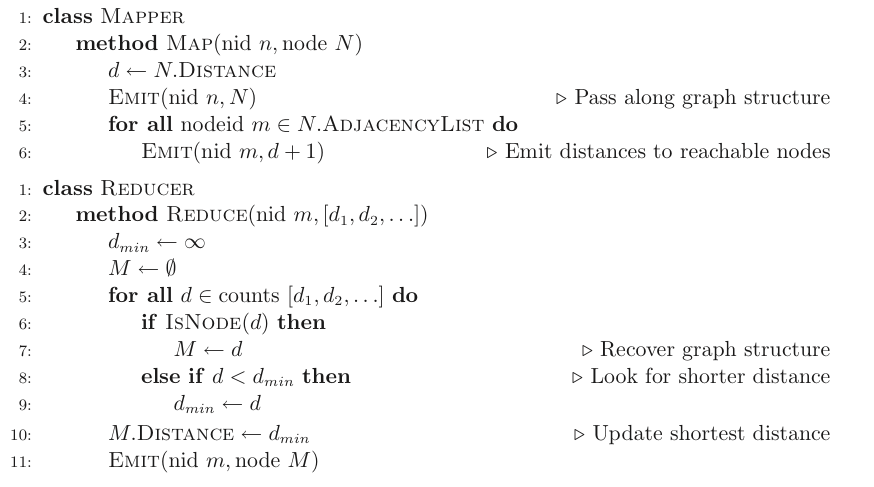
\includegraphics[scale=0.4]{./Figures/pbfs}
  \end{center}
}

%%%%%%%%%%%%%%%%%%%%%%%%%%%%%%%%%%%%%%%%%%%%%%%%%%%%%%%%%%
\frame {\frametitle{Parallel Breadth-First Search}
%%%%%%%%%%%%%%%%%%%%%%%%%%%%%%%%%%%%%%%%%%%%%%%%%%%%%%%%%%
  \begin{itemize}
  \item \textbf{Assumptions}
    \begin{itemize}
    \item Connected, directed graph
    \item Data structure: adjacency list
    \item Distance to each node is stored alongside the adjacency list
      of that node
    \end{itemize}

    \vspace{20pt}

  \item \textbf{The pseudo-code}
    \begin{itemize}
    \item We use $n$ to denote the node id (an integer)
    \item We use $N$ to denote the node adjacency list and current
      distance
    \item The algorithm works by mapping over all nodes
    \item Mappers emit a key-value pair for each neighbor on the
      node's adjacency list
      \begin{itemize}
      \item The key: node id of the neighbor
      \item The value: the current distance to the node plus one
      \item If we can reach node $n$ with a distance $d$, then we must
        be able to reach all the nodes connected to $n$ with distance $d+1$
      \end{itemize}
    \end{itemize}
  \end{itemize}
}

%%%%%%%%%%%%%%%%%%%%%%%%%%%%%%%%%%%%%%%%%%%%%%%%%%%%%%%%%%
\frame {\frametitle{Parallel Breadth-First Search}
%%%%%%%%%%%%%%%%%%%%%%%%%%%%%%%%%%%%%%%%%%%%%%%%%%%%%%%%%%
  \begin{itemize}
  \item \textbf{The pseudo-code (continued)}
    \begin{itemize}
    \item After shuffle and sort, reducers receive keys corresponding
      to the destination node ids and distances corresponding to all
      paths leading to that node
    \item The reducer selects the shortest of these distances and
      update the distance in the node data structure
    \end{itemize}

    \vspace{20pt}

  \item \textbf{Passing the graph along}
    \begin{itemize}
    \item The mapper: emits the node adjacency list, with the node id
      as the key
    \item The reducer: must distinguish between the node data
      structure and the distance values
    \end{itemize}
 \end{itemize}
}

%%%%%%%%%%%%%%%%%%%%%%%%%%%%%%%%%%%%%%%%%%%%%%%%%%%%%%%%%%
\frame {\frametitle{Parallel Breadth-First Search}
%%%%%%%%%%%%%%%%%%%%%%%%%%%%%%%%%%%%%%%%%%%%%%%%%%%%%%%%%%
  \begin{itemize}
  \item \textbf{MapReduce iterations}
    \begin{itemize}
    \item The first time we run the algorithm, we ``discover'' all
      nodes connected to the source
    \item The second iteration, we discover all nodes connected to
      those
    \item[$\to$] Each iteration expands the ``search frontier'' by one
      hop
    \item {\color{red}How many iterations before convergence?}
    \end{itemize}

    \vspace{40pt}

  \item \textbf{This approach is suitable for small-world graphs}
    \begin{itemize}
    \item The diameter of the network is small
    \item See \cite{Lattanzi2011} for advanced topics on the subject
    \end{itemize}
  \end{itemize}
}

%%%%%%%%%%%%%%%%%%%%%%%%%%%%%%%%%%%%%%%%%%%%%%%%%%%%%%%%%%
\frame {\frametitle{Parallel Breadth-First Search}
%%%%%%%%%%%%%%%%%%%%%%%%%%%%%%%%%%%%%%%%%%%%%%%%%%%%%%%%%%
  \begin{itemize}
  \item \textbf{Checking the termination of the algorithm}
    \begin{itemize}
    \item Requires a ``driver'' program which submits a job, check
      termination condition and eventually iterates
    \item In practice:
      \begin{itemize}
      \item Hadoop counters
      \item Side-data to be passed to the job configuration
      \end{itemize}
    \end{itemize}

    \vspace{40pt}

  \item \textbf{Extensions}
    \begin{itemize}
    \item Storing the actual shortest-path
    \item Weighted edges (as opposed to unit distance)
    \end{itemize}
  \end{itemize}
}

%%%%%%%%%%%%%%%%%%%%%%%%%%%%%%%%%%%%%%%%%%%%%%%%%%%%%%%%%%
\frame {\frametitle{The story so far}
%%%%%%%%%%%%%%%%%%%%%%%%%%%%%%%%%%%%%%%%%%%%%%%%%%%%%%%%%%
  \begin{itemize}
  \item \textbf{The graph structure is stored in an adjacency lists}
    \begin{itemize}
    \item This data structure can be augmented with additional information
    \end{itemize}

    \vspace{20pt}

  \item \textbf{The MapReduce framework}
    \begin{itemize}
    \item Maps over the node data structures involving only the node's
      internal state and it's {\color{red}local} graph structure
    \item Map results are ``passed'' along outgoing edges
    \item The graph itself is passed from the mapper to the reducer
      \begin{itemize}
      \item This is a very costly operation for large graphs!
      \end{itemize}
    \item Reducers aggregate over ``same destination'' nodes
    \end{itemize}

    \vspace{20pt}

  \item \textbf{Graph algorithms are generally iterative}
    \begin{itemize}
    \item Require a driver program to check for termination
    \end{itemize}
  \end{itemize}
}

%%%%%%%%%%%%%%%%%%%%%%%%%%%%%%%%%%%%%%%%%%%%%%%%%%%%%%%%%%
%%%%%%%%%%%%%%%%%%%%%%%%%%%%%%%%%%%%%%%%%%%%%%%%%%%%%%%%%%
\subsection{PageRank}
%%%%%%%%%%%%%%%%%%%%%%%%%%%%%%%%%%%%%%%%%%%%%%%%%%%%%%%%%%
%%%%%%%%%%%%%%%%%%%%%%%%%%%%%%%%%%%%%%%%%%%%%%%%%%%%%%%%%%

%%%%%%%%%%%%%%%%%%%%%%%%%%%%%%%%%%%%%%%%%%%%%%%%%%%%%%%%%%
\frame {\frametitle{Introduction}
%%%%%%%%%%%%%%%%%%%%%%%%%%%%%%%%%%%%%%%%%%%%%%%%%%%%%%%%%%
  \begin{itemize}
  \item \textbf{What is PageRank}
    \begin{itemize}
    \item It's a measure of the relevance of a Web page, based on the
      structure of the hyperlink graph
    \item Based on the concept of random Web surfer
    \end{itemize}

    \vspace{20pt}
  
  \item \textbf{Formally we have: }
    $$P(n) = \alpha \Big( \frac{1}{|G|}\Big) + (1-\alpha) \sum_{m \in L(n)}\frac{P(m)}{C(m)}$$
    \begin{itemize}
    \item $|G|$ is the number of nodes in the graph
    \item $\alpha$ is a random jump factor
    \item $L(n)$ is the set of out-going links from page $n$
    \item $C(m)$ is the out-degree of node $m$
    \end{itemize}
  \end{itemize}
}

%%%%%%%%%%%%%%%%%%%%%%%%%%%%%%%%%%%%%%%%%%%%%%%%%%%%%%%%%%
\frame {\frametitle{PageRank in Details}
%%%%%%%%%%%%%%%%%%%%%%%%%%%%%%%%%%%%%%%%%%%%%%%%%%%%%%%%%%
  \begin{itemize}
  \item \textbf{PageRank is defined recursively, hence we need an
      iterative algorithm}
    \begin{itemize}
    \item A node receives ``contributions'' from all pages that link
      to it
    \end{itemize}

    \vspace{20pt}
    
  \item \textbf{Consider the set of nodes $L(n)$}
    \begin{itemize}
    \item A random surfer at $m$ arrives at $n$ with probability
      $1/C(m)$
    \item Since the PageRank value of $m$ is the probability that the
      random surfer is at $m$, the probability of arriving at $n$ from
      $m$ is $P(m)/C(m)$
    \end{itemize}

    \vspace{20pt}

  \item \textbf{To compute the PageRank of $n$ we need:}
    \begin{itemize}
    \item Sum the contributions from all pages that link to $n$
    \item Take into account the random jump, which is uniform over all
      nodes in the graph
    \end{itemize}
  \end{itemize}
}

%%%%%%%%%%%%%%%%%%%%%%%%%%%%%%%%%%%%%%%%%%%%%%%%%%%%%%%%%%
\frame {\frametitle{PageRank in MapReduce}
%%%%%%%%%%%%%%%%%%%%%%%%%%%%%%%%%%%%%%%%%%%%%%%%%%%%%%%%%%
  \begin{center}
    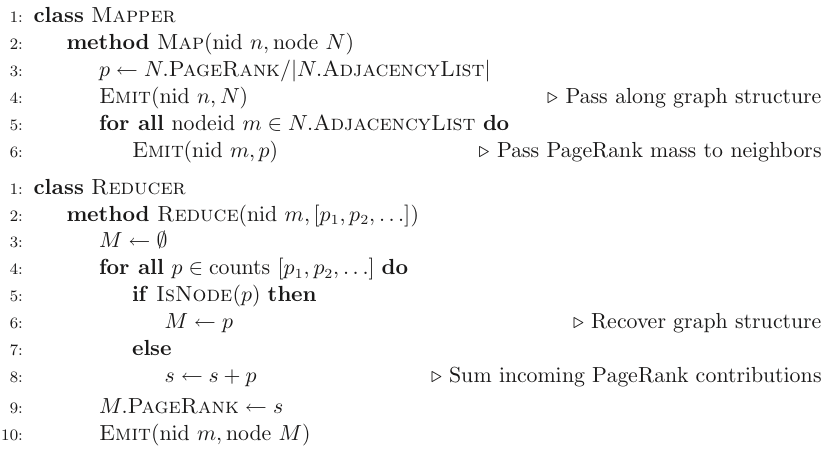
\includegraphics[scale=0.4]{./Figures/pr}
  \end{center}
}

%%%%%%%%%%%%%%%%%%%%%%%%%%%%%%%%%%%%%%%%%%%%%%%%%%%%%%%%%%
\frame {\frametitle{PageRank in MapReduce}
%%%%%%%%%%%%%%%%%%%%%%%%%%%%%%%%%%%%%%%%%%%%%%%%%%%%%%%%%%
  \begin{center}
    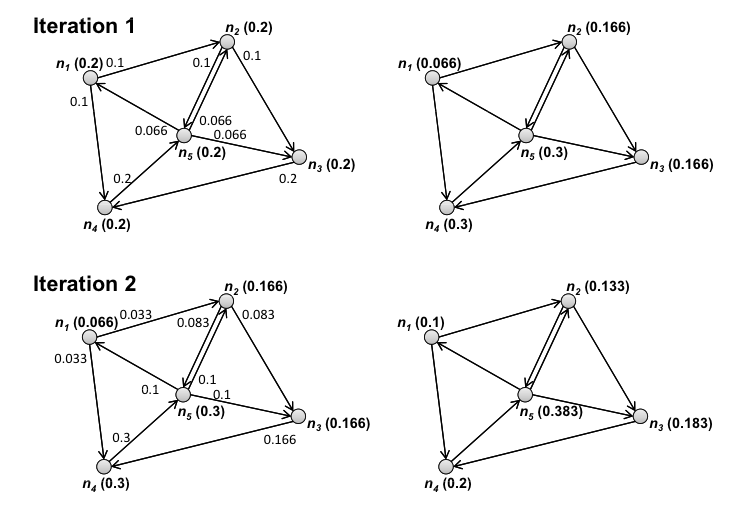
\includegraphics[scale=0.4]{./Figures/pr_toy}
  \end{center}
}

%%%%%%%%%%%%%%%%%%%%%%%%%%%%%%%%%%%%%%%%%%%%%%%%%%%%%%%%%%
\frame {\frametitle{PageRank in MapReduce}
%%%%%%%%%%%%%%%%%%%%%%%%%%%%%%%%%%%%%%%%%%%%%%%%%%%%%%%%%%
 \begin{center}
    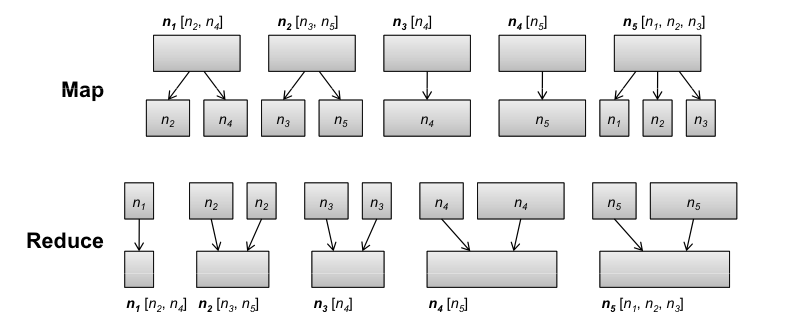
\includegraphics[scale=0.4]{./Figures/pr_sketch}
  \end{center}
}

%%%%%%%%%%%%%%%%%%%%%%%%%%%%%%%%%%%%%%%%%%%%%%%%%%%%%%%%%%
\frame {\frametitle{PageRank in MapReduce}
%%%%%%%%%%%%%%%%%%%%%%%%%%%%%%%%%%%%%%%%%%%%%%%%%%%%%%%%%%
  \begin{itemize}
  \item \textbf{Sketch of the MapReduce algorithm}
    \begin{itemize}
    \item The algorithm maps over the nodes
    \item For each node computes the PageRank mass the needs to be
      distributed to neighbors
    \item Each fraction of the PageRank mass is emitted as the value,
      keyed by the node ids of the neighbors
    \item In the shuffle and sort, values are grouped by node id
      \begin{itemize}
      \item Also, we pass the graph structure from mappers to reducers
        (for subsequent iterations to take place over the updated graph)
      \end{itemize}
    \item The reducer updates the value of the PageRank of every
      single node
    \end{itemize}
  \end{itemize}
}

%%%%%%%%%%%%%%%%%%%%%%%%%%%%%%%%%%%%%%%%%%%%%%%%%%%%%%%%%%
\frame {\frametitle{PageRank in MapReduce}
%%%%%%%%%%%%%%%%%%%%%%%%%%%%%%%%%%%%%%%%%%%%%%%%%%%%%%%%%%
  \begin{itemize}
  \item \textbf{Implementation details}
    \begin{itemize}
    \item Loss of PageRank mass for sink nodes
    \item Auxiliary state information
    \item One iteration of the algorithm
      \begin{itemize}
      \item Two MapReduce jobs: one to distribute the PageRank mass,
        the other for dangling nodes and random jumps
      \end{itemize}
    \item Checking for convergence
      \begin{itemize}
      \item Requires a driver program
      \item When updates of PageRank are ``stable'' the algorithm stops
      \end{itemize}
    \end{itemize}
    
    \vspace{20pt}
    
  \item \textbf{Further reading on {\color{red}convergence} and
      {\color{red}attacks}}
    \begin{itemize}
    \item Convergence: \cite{Page1999, Bianchini2005}
    \end{itemize}
  \end{itemize}
}

%%%%%%%%%%%%%%%%%%%%%%%%%%%%%%%%%%%%%%%%%%%%%%%%%%%%%%%%%%

%%%%%%%%%%%%%%%%%%%%%%%%%%%%%%%%%%%%%%%%%%%%%%%%%%%%%%%%%%
\section{References}

\begin{frame}
 \begin{colorblock}{blue}{lightblue}{ }
  \begin{center}
    \Huge \textbf{\texttt{References}}
  \end{center}
  \end{colorblock}
\end{frame}

\begin{frame}[allowframebreaks]{References}
\bibliographystyle{plain} 
\bibliography{references} 
\end{frame}
%%%%%%%%%%%%%%%%%%%%%%%%%%%%%%%%%%%%%%%%%%%%%%%%%%%%%%%%%%

\end{document}
